\normalfalse \difficiletrue \tdifficilefalse
\correctionfalse

%\UPSTIidClasse{11} % 11 sup, 12 spé
%\newcommand{\UPSTIidClasse}{12}

\exer{Tabouret  $\star\star$ \label{B2:12:513}}
\setcounter{question}{0}\UPSTIcompetence{B2-12}
\index{Compétence B2-12}

\ifcorrection
\else
\marginnote{\textbf{Pas de corrigé pour cet exercice.}}
\fi

\ifprof
\else
\begin{center}
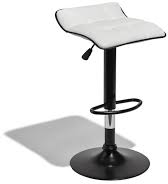
\includegraphics[width=.5\linewidth]{513_01}
\end{center}
\fi


\question{Proposer un schéma cinématique permettant de modéliser la liaison entre l'assise et le sol.}
\ifprof
\else
\fi

\ifprof
\else
\begin{flushright}
\footnotesize{Corrigé  voir \ref{B2:12:513}.}
\end{flushright}%
\fi